\begin{figure}[tbp]
    \centering
    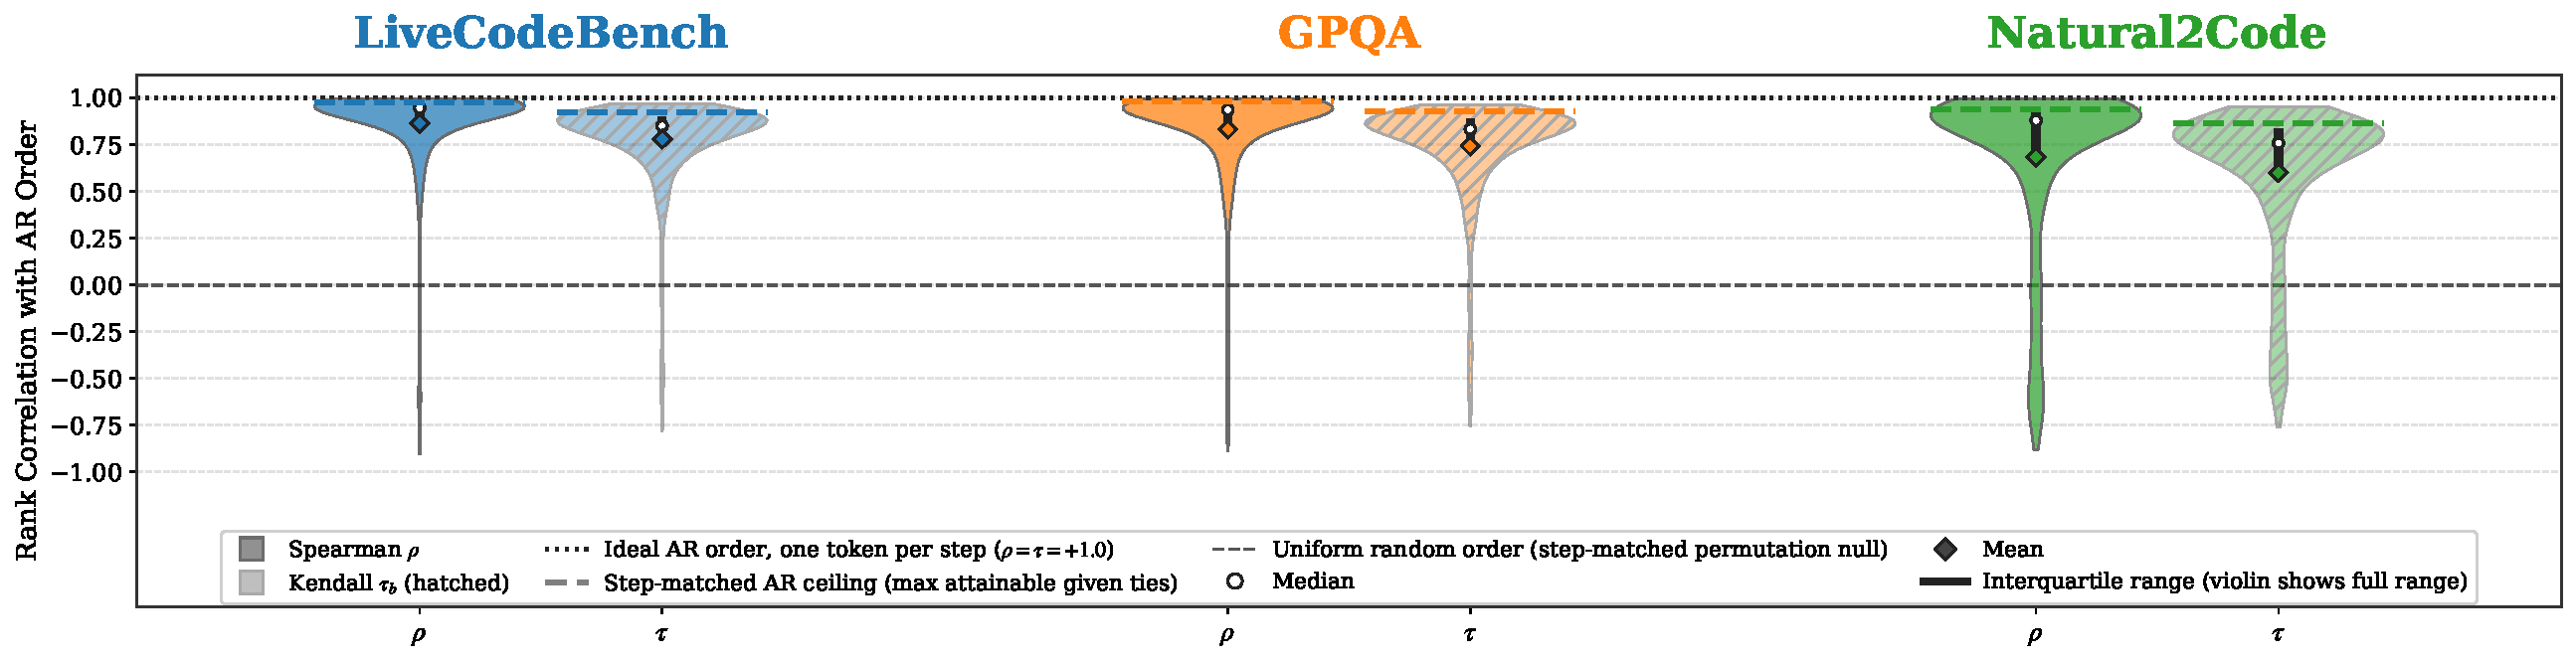
\includegraphics[width=\linewidth]{images/fig_ar_order_correlation_eb0.1_renoise.pdf}

    \vspace{8pt}

    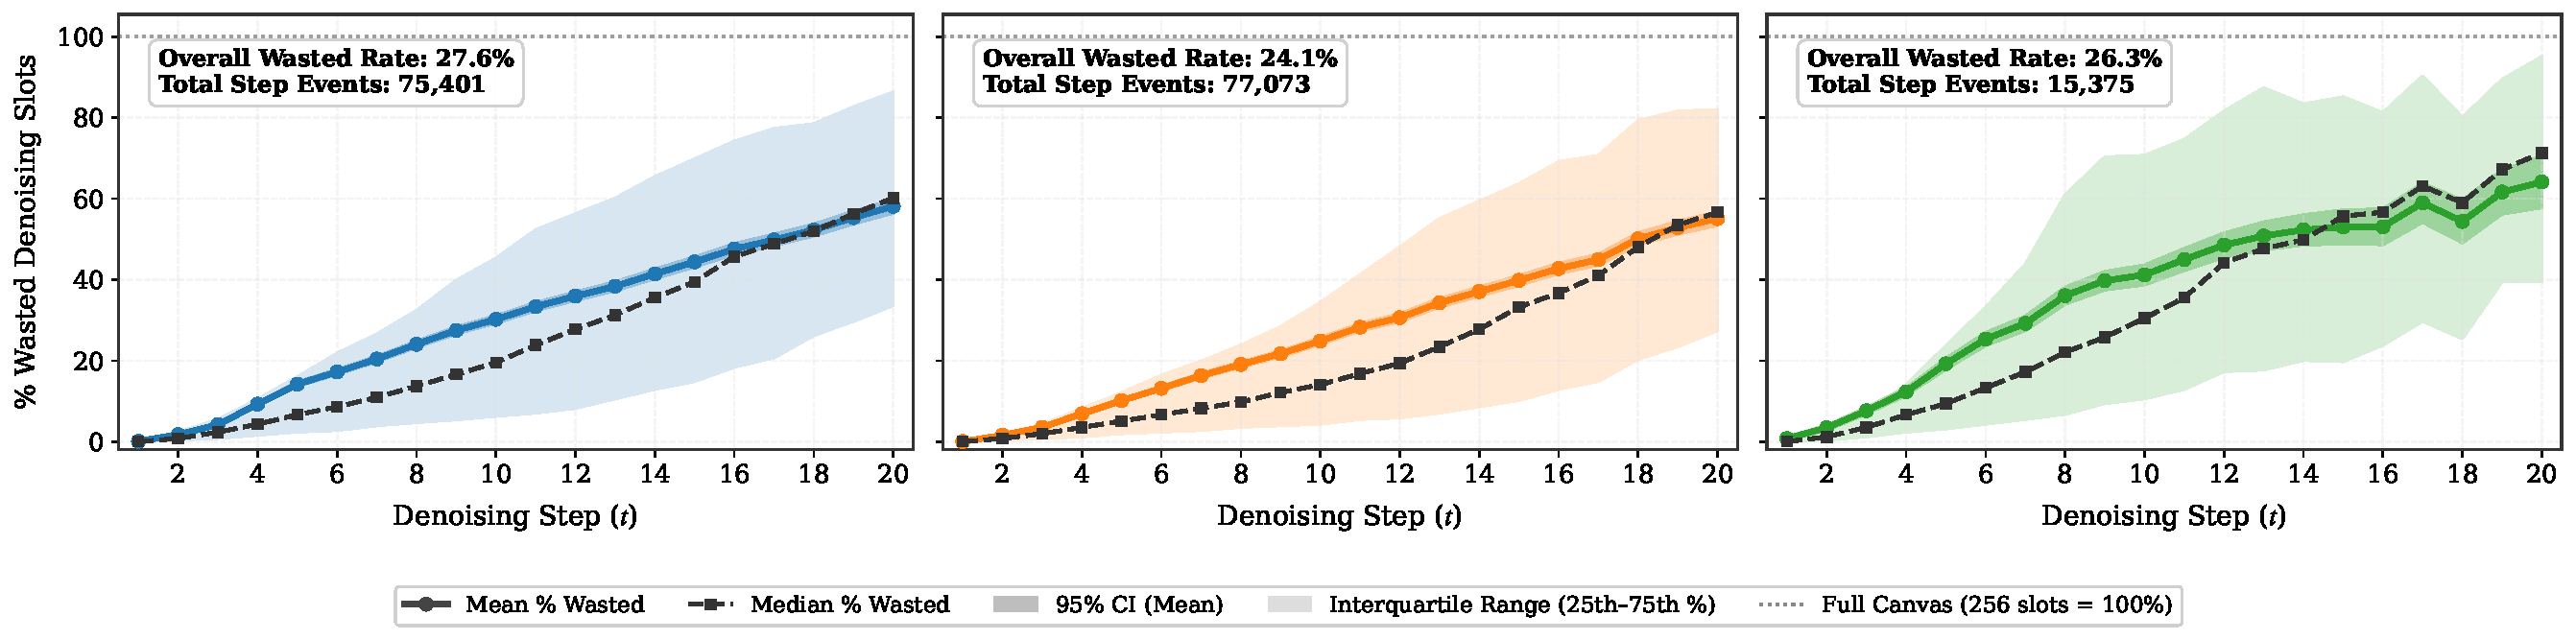
\includegraphics[width=\linewidth]{images/wasted_canvas_slots_lcb_gpqa_n2c.pdf}

    \vspace{8pt}

    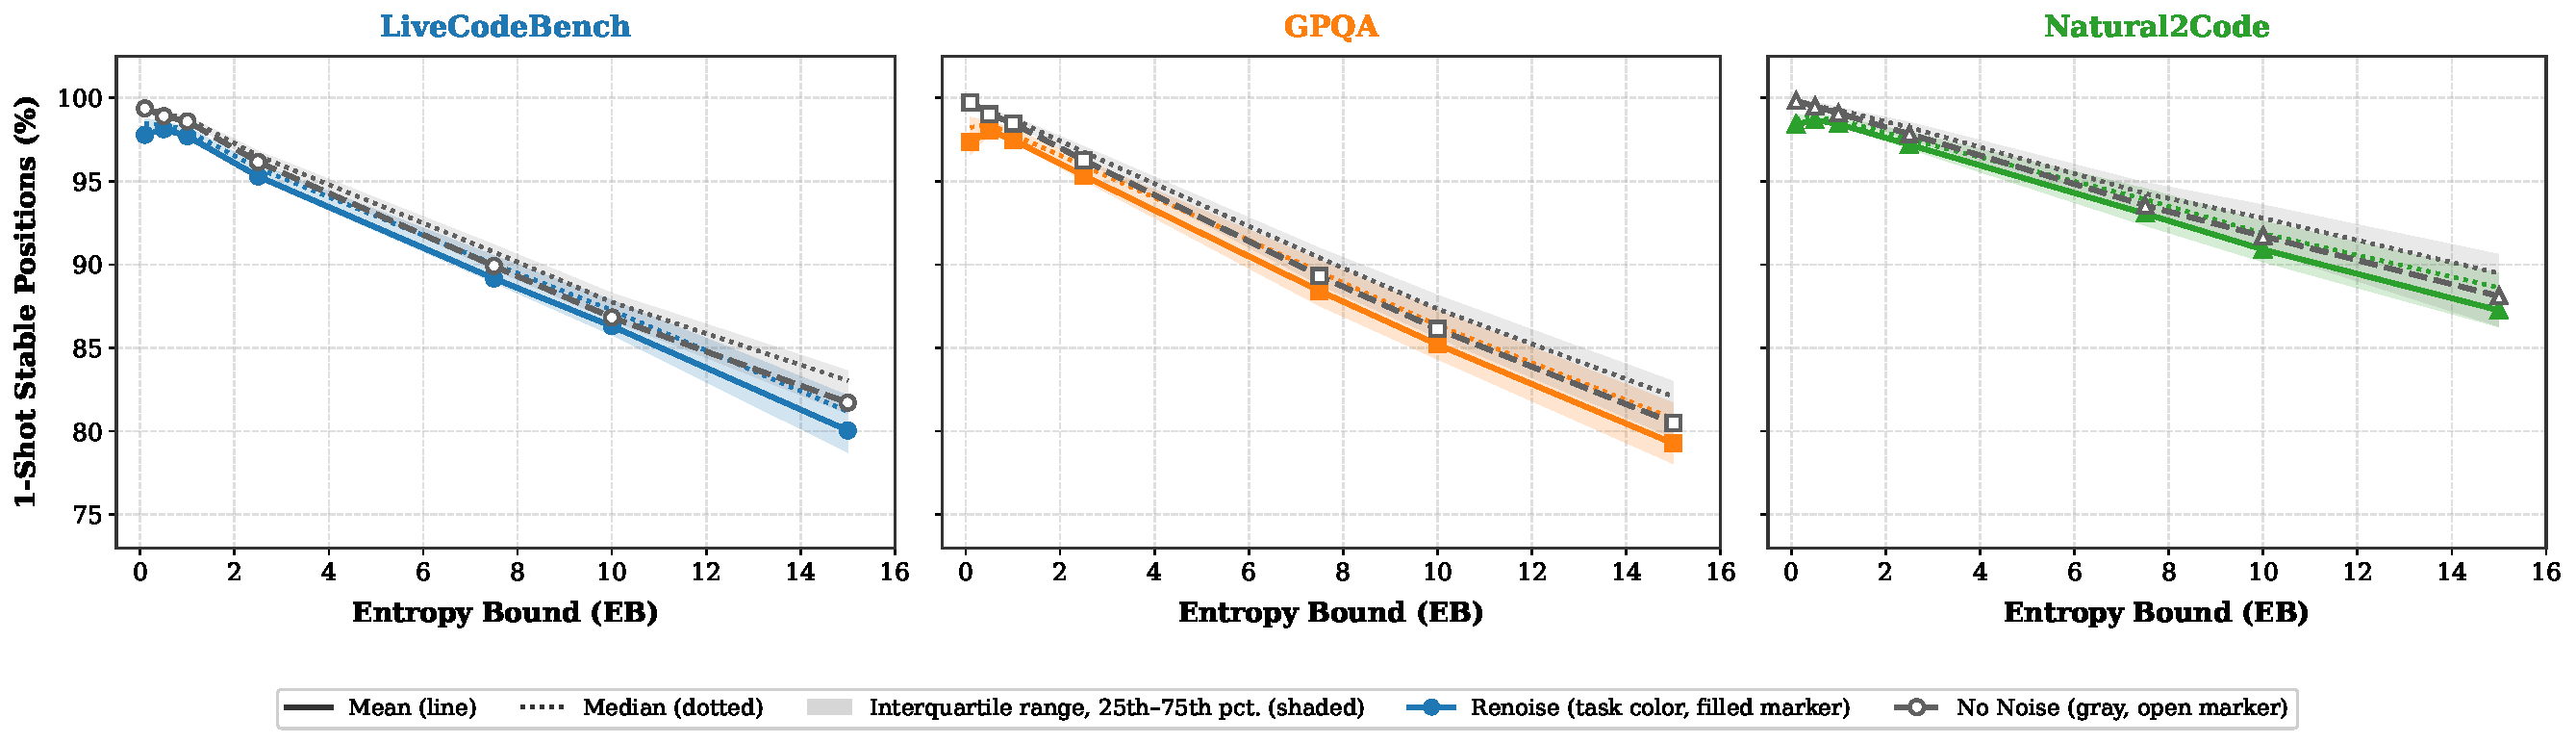
\includegraphics[width=\linewidth,trim=0 0 0 23.5pt,clip]{images/fig_1shot_stability_1x2_row.pdf}
    \caption{Columns show LiveCodeBench, GPQA Diamond, and Natural2Code in every row. \textbf{Top row:} Spearman $\rho$ and Kendall $\tau$ between the acceptance order of the DiffusionGemma EB sampler and the AR generation order; across all tasks the sampler is strongly biased towards left-to-right order. \textbf{Middle row:} Number of wasted denoising slots averaged across canvases for LCB v6, GPQA Diamond and Natural2Code. For a given sampling step, a slot is wasted if it belongs to a contiguous prefix that has already converged to its final token. Past 10 denoising steps, over half of the canvas slots are wasted. \textbf{Bottom row:} Accepted tokens are revised more often at higher entropy bounds (in both argmax and sampled-token stability), independent of renoising.}
    \label{fig:wasted}
\end{figure}
